\documentclass[a4paper,11pt]{article}

% Pacotes Principais -----------------------------------------------------------
\usepackage[portuges,brazil]{babel}
\usepackage[utf8]{inputenc}

% Figuras e Imagens ------------------------------------------------------------
\usepackage{graphicx}
% Figuras lado a lado
\usepackage{epsfig}
\usepackage{subfigure}

% Utilizar H para inserir as imagens REALMENTE onde eu desejo
\usepackage{float}

% Fontes -----------------------------------------------------------------------
\usepackage[T1]{fontenc}
\usepackage{pslatex}

% Simbolos ---------------------------------------------------------------------
\usepackage{textcomp}

% Tabelas ----------------------------------------------------------------------
%\usepackage{multicol}
\usepackage{multirow}
% Colorir a tabela
\usepackage{colortbl}

% Outros pacotes ---------------------------------------------------------------
\usepackage{noitemsep}

\usepackage{color}
\usepackage{xcolor}

% Comentários em bloco
\usepackage{verbatim}

% Sublinhado, traçado...
\usepackage{ulem}

% Desenhar
\usepackage{tikz}

% Comandos gerais --------------------------------------------------------------

% Configuração da fonte
\renewcommand{\familydefault}{\sfdefault}

% Comandos matemáticos ---------------------------------------------------------
% Implicação em fórmulas
\newcommand{\implica}{$\quad\Rightarrow\quad$} %Meio de linha
\newcommand{\implicafim}{$\quad\Rightarrow$}   %Fim de linha
\newcommand{\tende}{$\rightarrow$}

% Fração com parenteses
\newcommand{\pfrac}[2]{\parent{\frac{#1}{#2}}}

% Transformada de Laplace e transformada Z
\newcommand{\lapl}{\pounds}
\newcommand{\transfz}{\mathcal{Z}}

% Sequências
\newcommand{\sequencia}[4]{$#1_{#2}$, $#1_{#3}$, \ldots, $#1_{#4}$}

% Outros ----------------------------------------------------------------------
\newcommand{\chave}[1]{\left\{#1\right\}}
\newcommand{\colchete}[1]{\left[#1\right]}
\newcommand{\parent}[1]{\left(#1\right)}

\let\D\displaymath

\newtheorem{definicao}{Definição}
\newtheorem{exemplo}{Exemplo}
\newtheorem{lema}{Lema}
\newtheorem{observ}{Observação}
\newtheorem{teorema}{Teorema}

\newcommand{\defin}[1]{\begin{definicao}#1\end{definicao}}
\newcommand{\exemp}[1]{\begin{exemplo}#1\end{exemplo}}
\newcommand{\obs}[1]{\begin{observ}#1\end{observ}}

\newcommand{\pixel}{{\it pixel}}

% Tikz
\usetikzlibrary{matrix}


\begin{document}

\begin{table}[H]
\centering
\begin{tabular}{cl}
% Primeira Linha
\multirow{7}{*}
{

\includegraphics[width=1.65cm]{imgs/uern}
} & \\
& Governo do Estado do Rio Grande do Norte\\
% Segunda Linha
& Secretaria de Estado da Educação, da Cultural e dos Desportos -- SECD\\
% Terceira Linha
& {\sc Universidade do Estado do Rio Grande do Norte -- UERN}\\
% Quarta Linha
& Pró-Reitoria de Ensino e Graduação -- PROEG\\
% Quinta Linha
& Ciências da Computação -- 1\textordfeminine\ Avaliação (10 pontos)\\
& 
\end{tabular}
\end{table}

Aluno:

\vspace{0.25cm} 

Data: %\today

\section*{Questão 1 (2 pontos)}
Em nossas primeiras aulas, vimos o que seria {\bf sinal} e o que seria {\bf
informação}. Vimos também que qualquer tipo de informação, independentemente de
sua natureza (analógica ou digital) pode ser codificada em uma estrutura de
dados (mídia de representação). Com base nessas informações e no que foi visto
em sala de aula, responda os itens abaixo.

\begin{itemize}
\item[a)] Defina o que é um sinal e o que é informação.
\item[b)] Um sinal analógico com frequência de 4 MHz deve ser digitalizado em um
computador e transferido para outro. Considerando que cada amostra do sinal será
representada com 4 bits, calcule a taxa de transmissão mínima para que não haja
perda de informação.
\end{itemize}

\pagebreak

\section*{Questão 2 (2 pontos)}
De acordo com o que foi visto em sala, quando pessoas distintas mencionam o
termo {\bf multimídia}, talvez estejam se referindo a coisas diferentes.
Defina o que é multimídia e cite algumas das facilidades em se utilizar arquivos
multimídia.

\pagebreak

\section*{Questão 3 (2 pontos)}
Quando comentamos em sala sobre autoria multimídia, mostrou-se que, do ponto de
vista de ambiente operacional, um sítio é visto como uma coleção de arquivos
organizados em uma estrutura de pastas. Diferencie {\bf sítios estáticos} de
{\bf sítios dinâmicos} e identifique as duas formas em que os {\bf códigos
ativos} podem ser executados.
\pagebreak

\section*{Questão 4 (2 pontos)}
Vimos em sala de aula que a construção de um produto multimídia deve ser
realizada a partir de um projeto, o qual denominamos de {\bf projeto
multimídia}. Identifique os elementos que devem ser levados em consideração ao
se elaborar um projeto multimídia. Determine também as fases do modelo de {\bf
ciclo de vida} sugerido em sala de aula, explicando sucintamente o significado
de cada uma delas.
\pagebreak

\section*{Questão 5 (2 pontos)}
Sabemos que as cores podem ser representadas através de combinações lineares de
cores básicas, também denominadas de cores elementares ou cores primárias.
Considerando o {\bf modelo de cores RGB} e a representação de imagens no formato
matricial, responda os itens abaixo.

\begin{itemize}
    \item[a)] Explique como se dá a pigmentação dos {\it pixels} em um monitor
CRT convencional.
    \item[b)] Considere uma matriz de dimensão $M \times N$ tal como mostra a
Fig. \ref{fig:matriz}. Sabendo que cada célula da matriz representa um {\it
pixel} e que cada {\it pixel} é codificado através do modelo RGB com {\bf 1
Byte/cor}, qual será o tamanho do arquivo da imagem ({\bf em KBytes})
representada por essa matriz quando $M = 80$ e $N = 40$?
\end{itemize}

\begin{figure}[H]
\centering
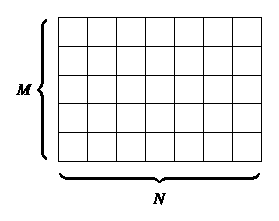
\includegraphics[width=0.3\textwidth]{imgs/matriz}
\caption{Matriz de {\it pixels} utilizada na Questão 5.}
\label{fig:matriz}
\end{figure}

\pagebreak

\section*{Questão 6 (1.0 ponto extra)}
Em um sistema de vídeo digital, deseja-se calcular a taxa de transmissão
necessária para realizar a transmissão de um sinal de vídeo sem que haja perda
de informação. Sabe-se que no protocolo de transmissão não há nenhum método de
verificação ou correção de erro. Ou seja, cada bit transmitido errado implicará
em retransmissão total do quadro. 

As especificações do sistema são:

\begin{itemize}
\item Resolução da tela de $640 \times 480$;
\item Quadros utilizam modelo de cor RGBA, sendo 1 Byte/Cor + 1 Byte de
transparência;
\item A taxa de atualização da tela é de 30 quadros/segundo (30 fps).
\end{itemize}

Com base nessas informações, responda:

\begin{itemize}
    \item [a)] Qual será a taxa de transmissão ({\bf em KBytes}) para atender as
especificações acima?
    \item [b)] Qual é o número de quadros transmitidos em 1 minuto de vídeo?
Qual volume de informação em GBytes?
    \item [c)] Supondo que a cada 90 quadros, 1 quadro é perdido (precisa ser
retransmitido), qual será o volume de dados em MBytes que precisará ser
retransmitido na transmissão de 1 minuto de vídeo?
\end{itemize}

\end{document}
